%\begin{itemize}
%	\item We show performance on the ``big tasks''(TIMIT, yearpred, CovType, Census, Adult).
%	\item We explain these results in terms of the ``small tasks'' (Census and Subsampled CovType), where we measure $\Delta$, showing that below a certain number of bits, $\Delta$ can increase a lot.  If we have space, we explain the trade-offs here a bit, showing in the fixed design setting that higher noise means higher $\lambda^*$, which means fewer bits can be used until $\Delta$ increases a lot.
%	\item We briefly present low-precision training, showing that performance doesn't degrade much relative to full-precision training.
%\end{itemize}
In this section, we empirically evaluate our generalization theory on low-precision RFF, and demonstrate the empirical generalization performance of low-precision RFF under memory budgets. On the Census dataset and subsampled Covtype, we first demonstrate the strong correlation of generalization performance and $\Delta$, which aligns with our $\Delta$ based bounds of generalization bound for low-precision RFF. We then extend to four different datasets, including the Census, YearPred dataset for kernel ridge regression and the Covtype, TIMIT dataset for kernel logistic regression. Across our experiment results, we compute the memory utilization as described in Section~\ref{subsec:memory_utils}.

\subsection{Strong correlation between generalization and $\Delta$\todo{Jian: need a english name for $\Delta$}}
Our theory in Section~\ref{sec:lprff} claims that in fixed design kernel ridge regression, the generalization performance strongly depends on the quantity $\Delta$.
To validate the strong correlation between generalization performance and the central quantity $\Delta$ in our generalization bound, we empirically show that the number of bits generating smaller $\Delta$ demonstrates better generalization performance. 
Specifically, we analyze the correlation on the Census dataset for kernel ridge regression. In addition, we demonstrate that this correlation from kernel ridge regression theory empirically generalize to kernel logistic regression. 

We solve the regression problem with closed form solution. In our experiment, we grid search the best-performing regularizer strength for the exact kernel; this best-performing regularizer strength is uniformly applied to all the different runs. For kernel logistic regression, we subsample 20k data points for both training and heldout set of the Covtype dataset to tractably compute $\Delta$. As there is no closed-form solution for logistic regression, we train with SGD using minibatch 250. We grid search the best performing learning rate and regularizer strength using 20k dimensional \Nystrom approximation as proxy to the optimal values for the exact kernel; the 20k dimensional \Nystrom approximation and the exact kernel share the same training kernel matrix. We grid search the regularizer strength from grid $\{1e^{-5}, 5e^{-5}, 1e^{-4}, 1e^{-3}, 5e^{-3}, 1e^{-2}, 5e^{-2}, 1e^{-1}\}$ for both task. The learning rate in logistic regression experiment is from the grid $\{5, 10, 50, 100\}$. We report the average $\Delta$ and the average generalization performance, along with the standard deviation, from 5 different random seeds.

In Figure~\ref{fig:generalizatio_col}, we can observe LP-RFF can achieve significantly smaller $\Delta$ and generalization performance than full precision RFF and \Nystrom. Specifically, 8 bits and 2 bit LP-RFF attains the optimal generalization performance for Census and Covtype respectively. Noticeably, on both the Census and the Covtype dataset, approximation configurations which have low $\Delta$ value also shows better generalization performance. The ordering with respect to $\Delta$ aligns well with the one with respect to generalization performance, demonstrating a strong correlation between $\Delta$ and generalization performance for approximated kernels.

\begin{figure}
	\centering
	\begin{tabular}{c c c c}
		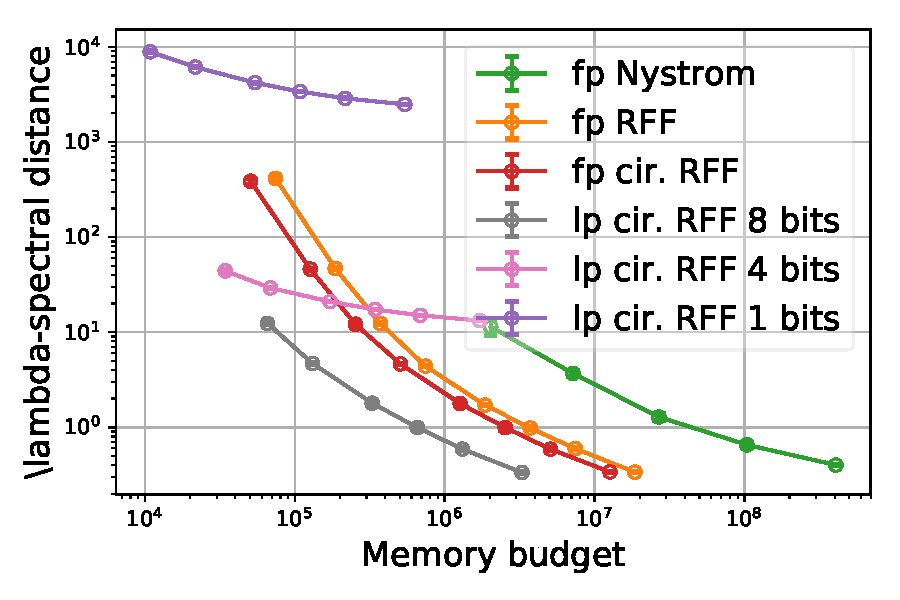
\includegraphics[width=0.24\linewidth]{figures/regression_delta_vs_mem.pdf} &
		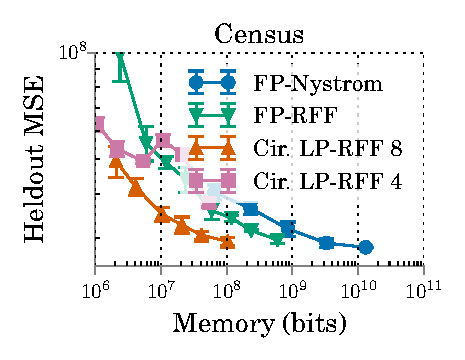
\includegraphics[width=0.24\linewidth]{figures/regression_l2_vs_mem.pdf} &
		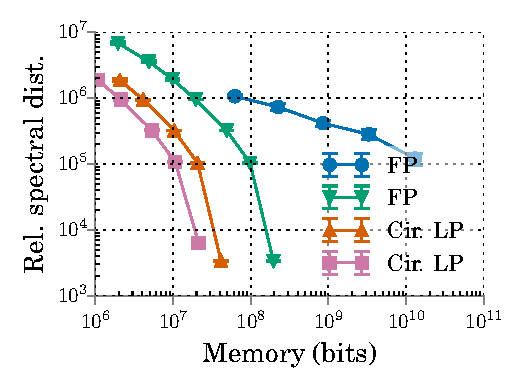
\includegraphics[width=0.24\linewidth]{figures/classification_delta_vs_mem.pdf} &
		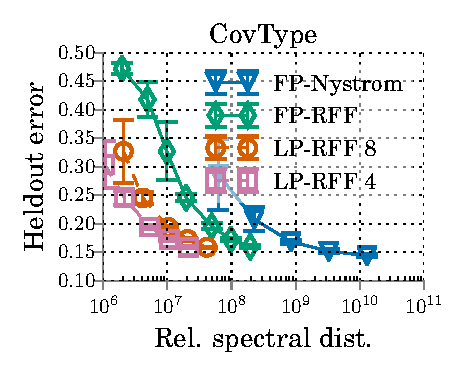
\includegraphics[width=0.24\linewidth]{figures/classification_acc_vs_mem.pdf} 
	\end{tabular}
	\caption{The strong correlation between generalization performance and $\Delta$ under memory budgets. Under different memory budget, the precision demonstrates smaller $\Delta$ tends to have better generalization performance.}
	\label{fig:generalizatio_col}
\end{figure}


\subsection{Generalization performance of low-precision random Fourier features}
To validate the generalization performance of LP RFF under memory budget, we compare LP RFF to FP RFF, FP circulant RFF and FP \Nystrom on larger datasets, showing the superior generalization performance of LP RFF under memory budget. 

In our experiments, we run \Nystrom method with up to $20000$ features while FP RFF, FP circulant RFF and LP RFF uses up to $400000$ features; the \Nystrom and FP RFF has similar memory consumption with the largest number of features. In this regime, it is computationally prohibitive to exhaustively grid search learning rate, L2 regularization and manually determine the number of training epochs for every configuration. Instead, we utilize early stopping across our experiments, which serves as regularization~\cite{wei2017early, zhang2005boosting} and determines the number of epochs automatically. Specifically, we use a vanilla early stopping rule. This rule drops the learning rate by a factor of 2 if the latest model can not provide more than $1\%$ improvement over the previous best model on heldout L2 loss for regression or heldout cross entropy for classification. The training process is terminated after the early stopping strategy drops learning rate for 10 ties. To fairly compare all approximation approach on each dataset, we use a uniform initial learning rate for SGD on this dataset for all different number of features. We grid search this uniform learning rate using $20\text{k}$ \Nystrom features, with the picked value optimizes heldout L2 loss for regression and heldout cross entropy for classification. We carry out the learning rate grid search using \Nystrom features to avoid biasing to better performance for RFF-based approximation approaches. 

We collect the generalization performance of LP RFF using $\{1,2,4,8,16\}$ bits, and quantitatively report \emph{memory saving} to measure the memory utilization improvement of LP RFF over baselines. Specifically, with a certain reference generalization performance from one baseline approach, we measure the minimal memory consumption of LP RFF across different number of bits to achieve within $1e^{-4}$ relative degradation to the reference. The \emph{memory saving} is defined as the ratio between the memory consumption of the reference performance and the minimal consumption from LP RFF. We measure the averaged memory saving with 3 runs using different random seeds, eliminating the fluctuation from a specific random seed. We report memory saving with respect to both the best and median heldout L2 loss or heldout accuracy from the feature number grid of baselines; this avoids the gain being inflated from the performance plateau near the best heldout metric.



\begin{figure}
	\centering
	\begin{tabular}{c c c c}
		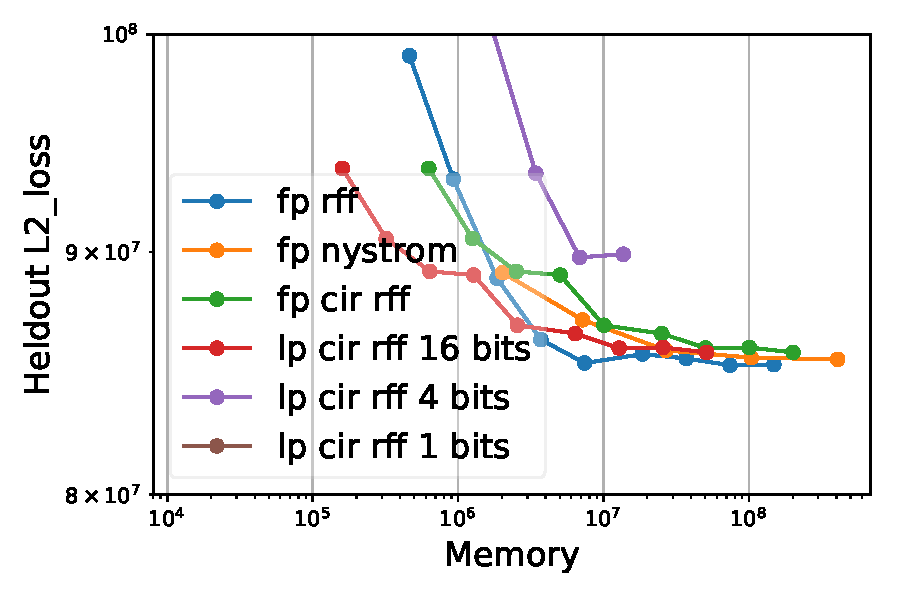
\includegraphics[width=0.24\linewidth]{figures/census_L2_loss_vs_n_memory.pdf} &
		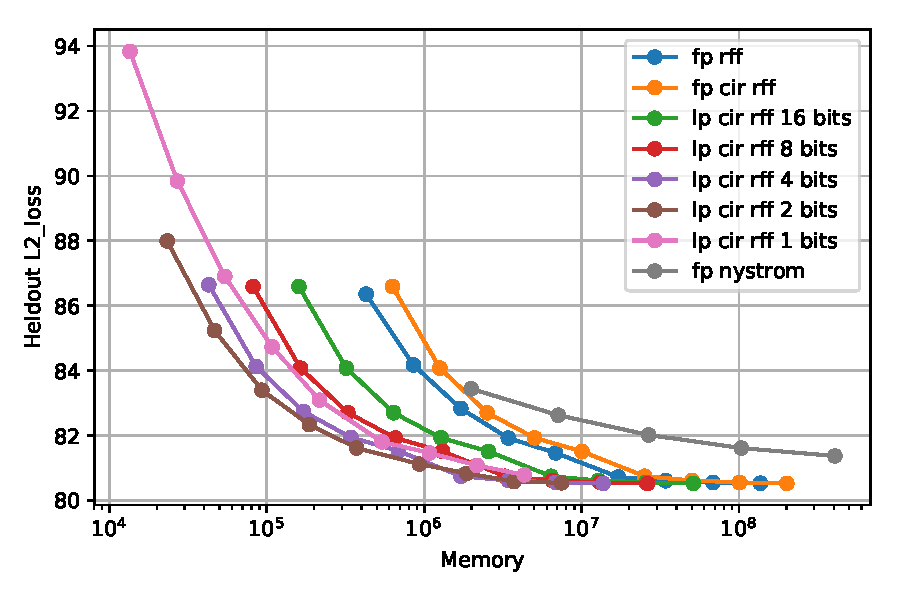
\includegraphics[width=0.24\linewidth]{figures/yearpred_L2_loss_vs_n_memory.pdf} &
		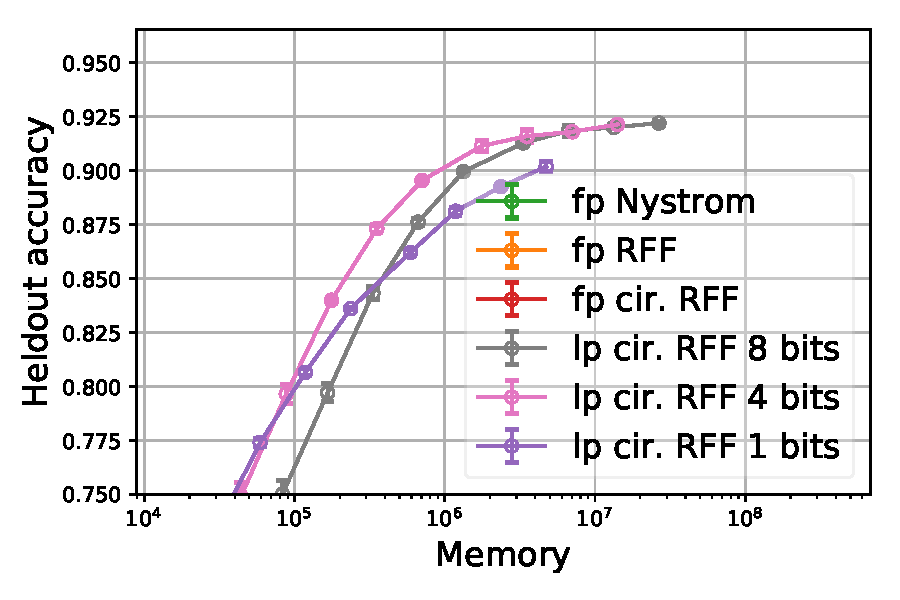
\includegraphics[width=0.24\linewidth]{figures/covtype_accuracy_vs_n_memory.pdf} &
		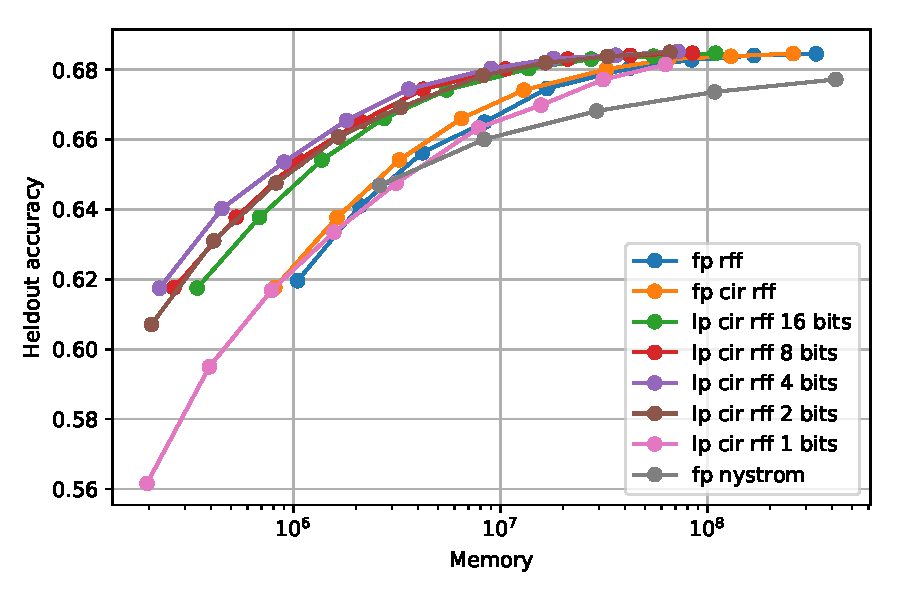
\includegraphics[width=0.24\linewidth]{figures/timit_accuracy_vs_n_memory.pdf} \\
		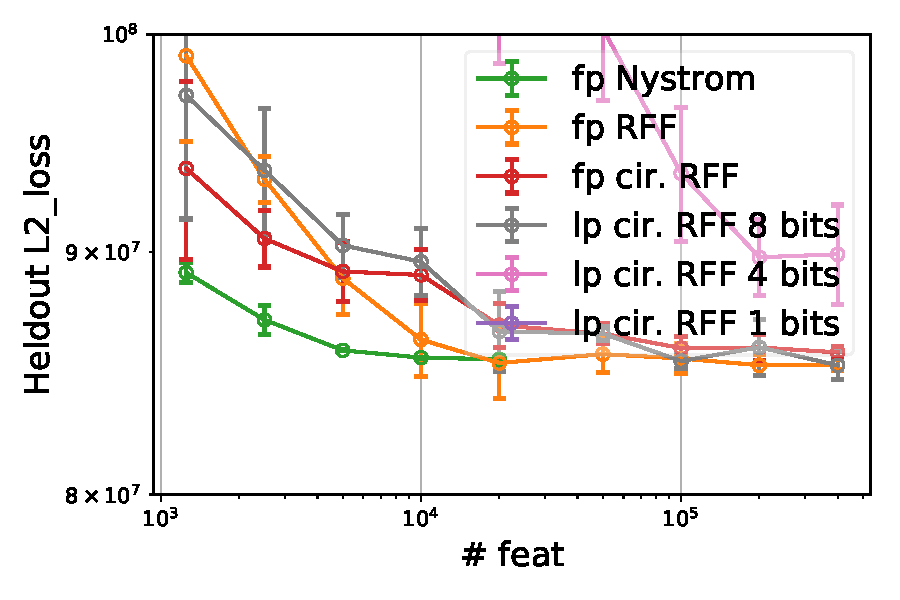
\includegraphics[width=0.24\linewidth]{figures/census_L2_loss_vs_n_feat.pdf} &
		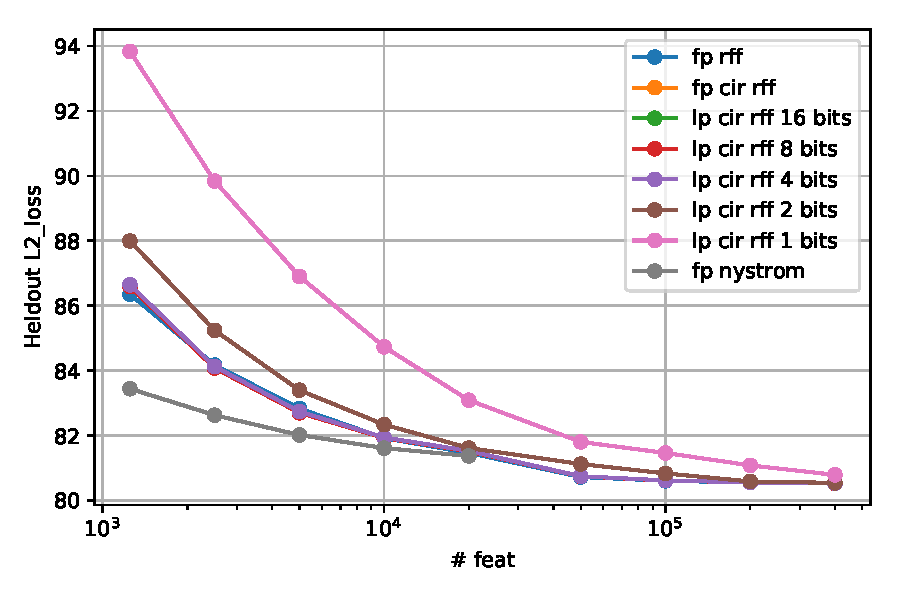
\includegraphics[width=0.24\linewidth]{figures/yearpred_L2_loss_vs_n_feat.pdf} &
		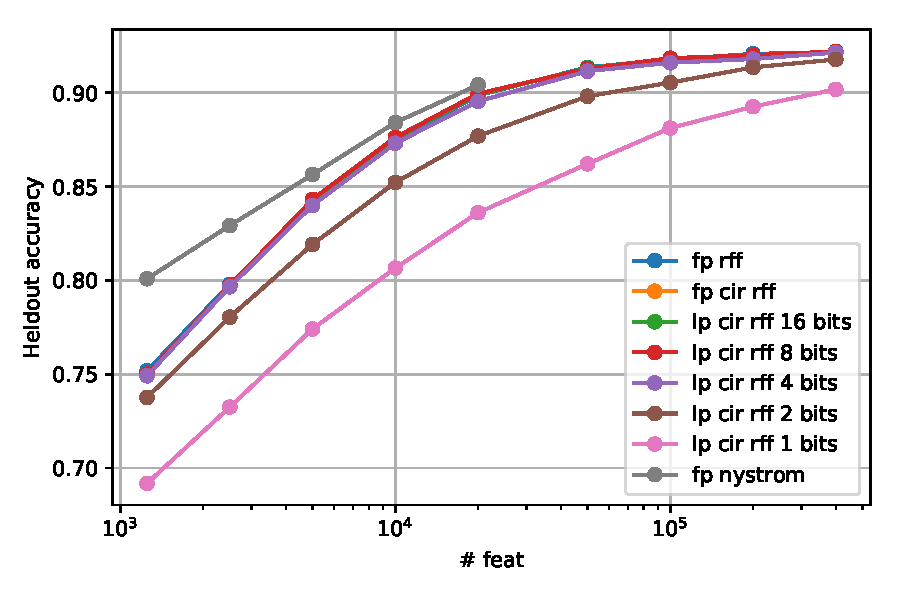
\includegraphics[width=0.24\linewidth]{figures/covtype_accuracy_vs_n_feat.pdf} &
		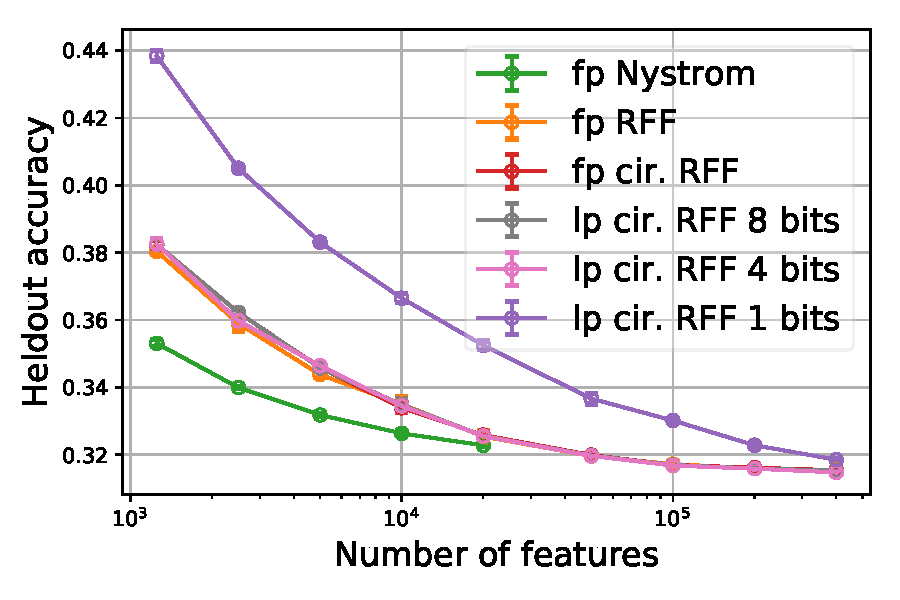
\includegraphics[width=0.24\linewidth]{figures/timit_accuracy_vs_n_feat.pdf} \\
		(a) Census & (b) YearPred & (c) Covtype & (d) TIMIT \\
	\end{tabular}
	\caption{Generalization performance of low precision RFF, full precision RFF and \Nystrom with respect to number of features and memory budgets.}
	\label{fig:generalizatio_col}
\end{figure}

%% version with out model memory
%\begin{table}
%	\centering
%	\begin{tabular}{c c c c}
%		\hline
%		& FP RFF & FP circulant RFF & \Nystrom \\
%		\hline
%		\hline
%		Census & 5.56x & 30.32x & 122.52x \\
%		YearPred & 19.35x & 14.30x & 829.15x \\ 
%		Covtype & 9.17x & 7.57x & 460.80x \\ 
%		TIMIT & 70.42x & 25.68x & 843.41x \\ 
%		\hline
%	\end{tabular}
%	\caption{The memory savings from LP RFF to achieve within $1e^{-4}$ relative difference from the best generalization performance of baselines. We measure heldout L2 loss and heldout accuracy as the generalization performance respectively for regression and classification problems.}
%	\label{fig:mem_saving}
%\end{table}

% version with model memory
\begin{table}
	\centering
	\begin{tabular}{c c c c}
		\hline
		& FP RFF & FP circulant RFF & \Nystrom \\
		\hline
		\hline
		Census & 2.8x/ & 30.7x/ & 62.2x/ \\
		YearPred & 9.99x/ & 14.7x/ & 436.9x/ \\ 
		Covtype & 4.6x/ & 7.6x/ & 230.4x/ \\ 
		TIMIT & 5.1x/ & 3.9x/ & 50.6x/ \\ 
		\hline
	\end{tabular}
	\caption{The memory savings from LP RFF to achieve within $1e^{-4}$ relative difference from reference performance of baselines. We measure heldout L2 loss and heldout accuracy as the generalization performance respectively for regression and classification problems. The memory saving is reported with respect to both the best and median performance from the feature number grid of a baseline; this avoids the gain being inflated from the performance plateau near the best heldout metric. }
	\label{fig:mem_saving}
\end{table}